\section{Charaktere und Items im Spiel}\label{sec:charactersAndItems}
Neben den statischen Level-Elementen benötigt es noch Charaktere in Form von Gegnern und dem Spieler selbst, die sich darauf fortbewegen können. Wie diese grundlegend aufgebaut sind, wird in Abschnitt \ref{sec:charactersBasic} dargestellt. Dabei wird insbesondere auch auf den Spieler und die zugehörige Benutzeroberfläche für den Endnutzer eingegangen. Da die konkrete Umsetzung der Gegner eine umfangreiche Thematik ist, wird dies separat in Kapitel \ref{sec:enemiesAndAI} behandelt.

Im Folgenden wird außerdem erläutert, wie interagierbare Gegenstände, also vornehmlich Waffen, in das Spiel integriert sind.

\subsection{Grundaufbau von Charakteren im Spiel}\label{sec:charactersBasic}
Auch wenn der Spieler und die Gegner sich in ihrer Funktionsweise stark unterscheiden, besitzen beide auch einige gemeinsame Eigenschaften. Aus diesem Grund erben sowohl der Spieler, als auch die Gegner von \texttt{Person} (siehe Abbildung \ref{fig:person_structure}). Jeder Charakter besitzt somit eine Anzahl an Lebenspunkten und Parameter zur Einstellung des Laufverhaltens, also zum Beispiel die Maximalgeschwindigkeit oder Beschleunigung der Person. Durch Implementierung des \texttt{IDamageable}-Interfaces ist es möglich jeder Person beispielsweise durch ein Projektil Schaden zufügen zu können. Die \texttt{Damage(...)}-Methode erhält dabei als Eingabeparameter die Anzahl an Schaden in Form von Lebenspunkten und eine Referenz auf das schadensverursachende Spielobjekt. Letzteres ist nötig, um zu erkennen, ob zum Beispiel bei Gegnern der Schaden von einem anderen Gegner verursacht wurde, und somit ignoriert werden soll.

\begin{figure}[h]
 \centering
 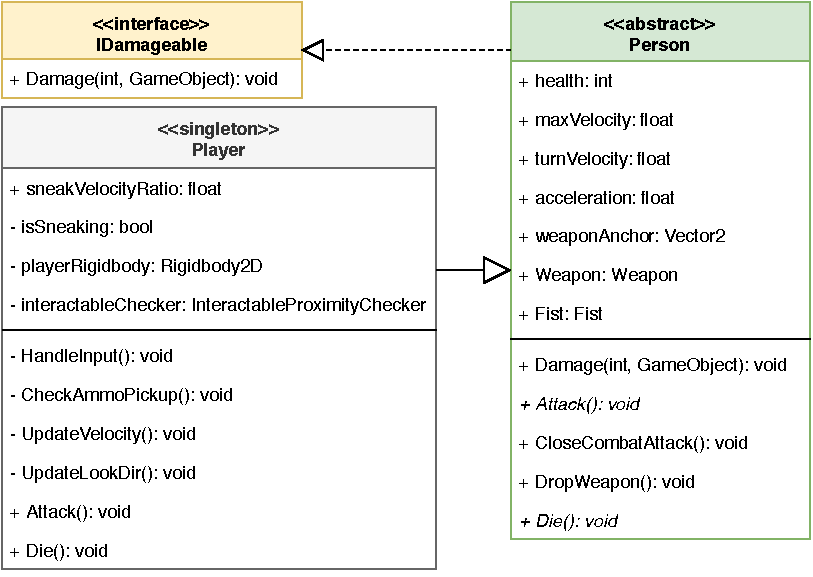
\includegraphics[width=0.8\linewidth]{diagrams/characters_reduced_UML.pdf}
 \captionof{figure}[Grundaufbau von Charakteren]{Vereinfachtes UML-Klassendiagramm der \texttt{Person}-Klasse und des Spielers}.
	\label{fig:person_structure}
\end{figure}

In der Klasse \texttt{Person} existiert zusätzlich je eine Referenz auf eine Waffe und eine Faust, die für Attacken genutzt werden können. Die Faust dient dabei zur Verwendung in Nahkampfangriffen über Aufruf der Methode \texttt{CloseCombatAttack()}, für den Fall, dass die Person aktuell keine andere Waffe besitzt. Sowohl die Klasse \texttt{Fist}, als auch \texttt{Weapon}, werden später in Abschnitt \ref{sec:weaponImplementation} genauer erklärt. Der \texttt{weaponAnchor} gibt noch an, in welchem räumlichen Versatz eine getragene Waffe zum Spielobjekt der Person platziert werden soll. Über die \texttt{DropWeapon()}-Methode kann ein Charakter dazu veranlasst werden seine aktuelle Waffe auf den Boden fallen zu lassen.

Alle Unterklassen von \texttt{Person} müssen außerdem die Angriffsmethode und die Methode \texttt{Die()} implementieren. Letztere wird aufgerufen, sobald die Anzahl der Lebenspunkte unter den Wert eins fällt.

Ähnlich wie für das Level, existiert hier ein sogenannter \texttt{PersonController}, der die Personen auf dem Level verwaltet. Er ermöglicht Zugriff auf die Charaktere im Level und ist bei Levelstart für deren Instanziierung zuständig. Dies geschieht unter Verwendung entsprechender Fabrikmethoden, die über \textit{Prefabs} Spielobjekte in der Szene erzeugen und mit den korrekten Parametern, wie unter anderem deren Position aufsetzen.

\subsubsection{Umsetzung des Spielers und dessen Steuerung}\label{sec:player}
Der Spieler, der schließlich vom Nutzer gesteuert wird, ist eine konkrete Implementierung der \texttt{Person}-Klasse und kann maximal einmal pro Szene in Unity existieren, wie in Abbildung \ref{fig:person_structure} zu sehen ist.

Bei jedem Aufruf der \texttt{Update()}-Methode der Unity-Engine werden über die \texttt{HandleInput()}-Methode die Nutzereingaben zur Steuerung des Spielers verarbeitet. Über die Tasten "`W"', "`A"', "`S"' und "`D"' oder die Pfeiltasten lässt sich der Spieler bewegen. Dabei wird der \textit{Rigidbody2D} des Spielers je nach den gedrückten Tasten in die entsprechende Richtung beschleunigt, bis die Maximalgeschwindigkeit erreicht ist. Der Spieler kann dabei zusätzlich bei gehaltener "`Shift"'-Taste schleichen. Dabei bewegt er sich zwar um den Faktor der \texttt{sneakVelocityRatio} langsamer, erzeugt beim Laufen allerdings keine Geräusche mehr, wodurch Gegner, wie in Kapitel \ref{sec:gegnerreaktionaufaudio} genauer beschrieben wird, den Spieler nicht mehr hören können. Zum Zielen dreht sich der Spieler durch Aufruf der \texttt{UpdateLookDir()}-Methode automatisch in die aktuelle Richtung des Mauszeigers.

Die \texttt{Player}-Klasse hält zudem eine Referenz auf einen \texttt{InteractableProximityChecker}. Dies ist eine Hilfsklasse, die dem Spielobjekt des Spielers als Komponente angefügt ist. Diese prüft zyklisch, welche interagierbaren Gegenstände im unmittelbaren Umkreis sind und hebt, sofern vorhanden, den nächsten Gegenstand farblich hervor. Über "`E"' kann der Spieler mit dem nächsten Gegenstand interagieren, also zum Beispiel eine Waffe aufheben. Mit "`Q"' kann eine Waffe zudem wieder fallen gelassen werden. Der \texttt{interactableChecker} wird außerdem verwendet, um automatisch Waffen aufzuheben, wenn sie vom gleichen Typ der aktuellen Waffe sind, um dann deren Munition zur aktuellen hinzuzufügen.

Bei Eliminierung des Spielers wird das aktuelle Level schließlich beendet und der Nutzer kann das Level neu starten, oder ins Hauptmenü zurückkehren.

\subsubsection{Die Benutzeroberfläche des Spielers}\label{sec:uiPlayer}
Um den Spieler die nötigen Informationen zur aktuellen Spielsituation zu vermitteln, wurde eine entsprechende Nutzeroberfläche eingebaut. Hierzu wird in der linken unteren Ecke der Szene die aktuelle Munitionsmenge angezeigt und rechts die Lebenspunkte des Spielers. Da das Spiel auch gewonnen werden kann, indem alle Gegner eliminiert werden, wird zudem in der linken oberen Ecke der Benutzeroberfläche die Anzahl verbleibender Gegner angezeigt, um so die Suche zu erleichtern.

\begin{figure}[h]
 \centering
 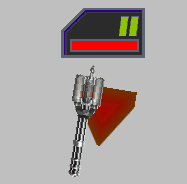
\includegraphics[width=0.2\linewidth]{pics/enemy_hud.PNG}
 \captionof{figure}[Informationsanzeige eines Gegners]{Informationsanzeige eines Gegners mit Lebens- und Aufmerksamkeitsbalken.}
	\label{fig:enemy_hud}
\end{figure}

Der Spieler benötigt zudem Informationen zum Status der einzelnen Gegner. Zu diesem Zwecke befindet sich oberhalb eines jeden Gegners eine entsprechende Anzeige, wie in Abbildung \ref{fig:enemy_hud} zu sehen. Diese zeigt zum einen, ähnlich wie beim Spieler, in Form von grünen Balken die aktuellen Lebenspunkte an. Zum anderen wird im unteren Balken die Spieleraufmerksamkeit des Gegners angezeigt, die angibt, inwieweit die Position des Spielers dem Gegner bekannt ist. Wurde der Spieler entdeckt, wird der Balken rot. Das darunterliegende Aufmerksamkeitssystem der Gegner wird in Kapitel \ref{sec:enemyImplementationAwareness} noch genau behandelt.

\subsection{Interaktive Gegenstände im Spiel}
\label{sec:weapon}

Neben den Level-Elementen und Charakteren spielen auch interaktive Gegenstände (engl. \textit{items}) eine wichtige Rolle. Diese beschränken sich zunächst auf Waffen, aber es wären auch weitere Gegenstände, beispielsweise Munition für die Waffen oder Gegenstände für die Wiederherstellung von Lebenspunkten denkbar.

\subsubsection{Design der Waffen}
\label{sec:weaponDesign}

Die Waffen im Spiel lassen sich in Nahkampf- und Fernkampfwaffen einteilen. Zu den Nahkampfwaffen gehören der Schlagstock sowie die Faust, welche als Unterobjekt jedes Charakters mitinstanziiert wird und zu den Fernkampfwaffen zählen die Pistole, das Maschinengewehr und die Schrotflinte.

Für alle Waffen außer der Faust, die aufgrund der Darstellung der Charaktere als farbige Pfeile unsichtbar ist, gibt es zwei Ansichten: Eine Ansicht von der Seite für im Level abgelegte Gegenstände, und eine von oben, für Gegenstände, die von einem Charakter getragen werden. Für jede dieser Waffen wurde für jede Ansicht ein Bild entweder selbst erstellt oder aus dem Internet ausgewählt und abgeändert (siehe \cite{Sprite_Machinegun} \cite{Sprite_Shotgun} \cite{Sprite_Bat}).

Damit Charaktere am anderen Ende des Levels nicht von Munition getroffen werden können, haben die Patronen eine relativ kurze Lebensdauer, die für jede Munitionssorte separat definiert wird.

\subsubsection{Implementierung der Waffen}
\label{sec:weaponImplementation}

Das gemeinsame Verhalten der Waffen ist in der abstrakten \texttt{Weapon}-Klasse definiert, welche die Interfaces \texttt{Item} und \texttt{IInteractable} implementiert. Von der \texttt{Weapon}-Klasse erben, wie in Abbildung \ref{fig:weaponStructure} gezeigt, wiederum die ebenfalls abstrakten Klassen \texttt{MeleeWeapon} für Nahkampfwaffen und \texttt{FireArm} für Fernkampfwaffen.

Jedem Waffen-\textit{Prefab} ist ein Projektil-\textit{Prefab} zugeordnet, welches in der \texttt{Fire()}-Methode der Waffe instanziiert wird. Dabei wird das Spielobjekt des Charakters, an dem die Waffe hängt, als \texttt{origin} des Projektils übergeben. Trifft der \textit{Collider} des Projektils auf den \textit{Collider} eines Spielcharakters, kann überprüft werden, ob der getroffene Charakter mit dem Ursprung des Projektils identisch ist. Ist dies nicht der Fall, wird die \texttt{Damage(...)} Methode der Person aufgerufen.

\begin{figure}[h]
 \centering
 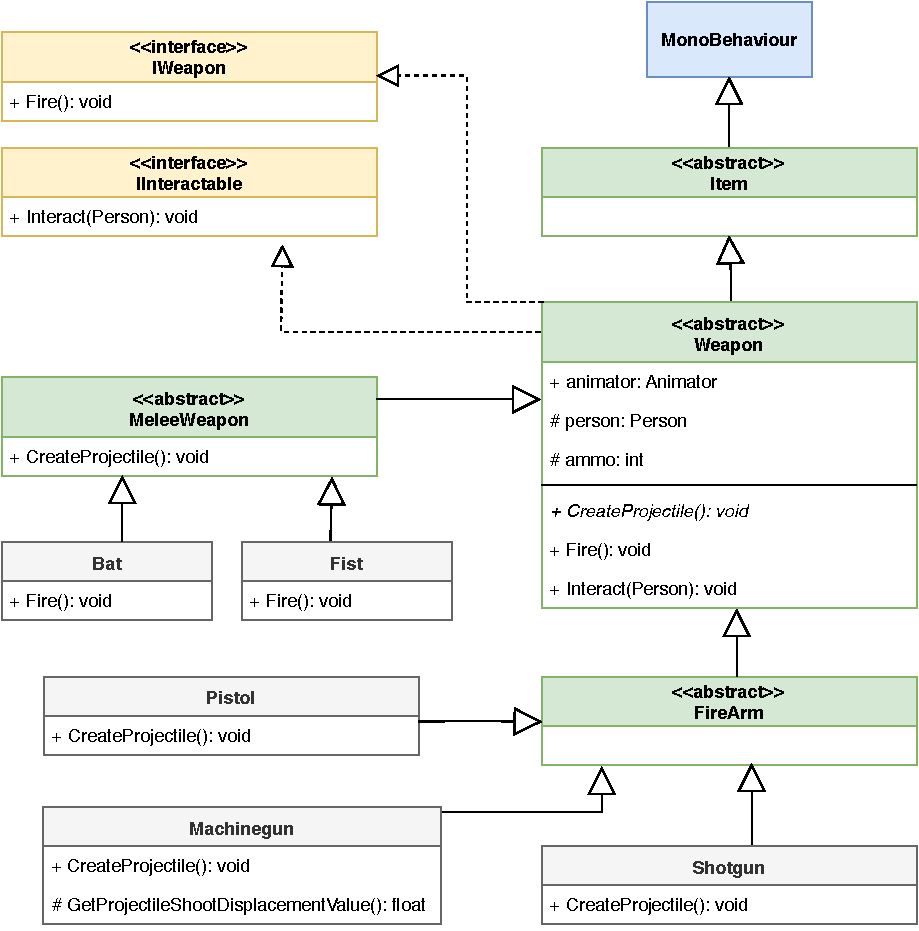
\includegraphics[width=0.835\linewidth]{diagrams/Weapon_Structure_reduced.pdf}
 \captionof{figure}[Datenstruktur der Waffen]{UML-Klassendiagramm der Waffen in reduzierter Darstellung}
	\label{fig:weaponStructure}
\end{figure}

Damit beim Aufnehmen und Ablegen von Waffen das \textit{Sprite} geändert wird, hat jeder Waffentyp außerdem einen entsprechenden \textit{Animator} (siehe Kapitel \ref{sec:unityGrafics}), durch den bei einer Änderung an seiner \texttt{onFloor} Variable eine Animation ausgeführt wird.
